\documentclass{beamer}
\usetheme{CambridgeUS}
\usecolortheme{wolverine}

\title{EE2227 PRESENTATION-1}
\author{D.SIVANI }
\institute{EE18BTECH11012}
\centering
\date{12 February 2020}
\begin{document}
\maketitle
\begin{frame}{Content}
\begin{itemize}
\item 2018 GATE paper(EE section) 
\item Question No:9

\end{itemize}
\end{frame}
\begin{frame}{Question}
\question  Match the transfer functions of the second-order systems with the nature of the systems given below
\newline \underline{Transfer functions}
\hspace{50mm}
\underline{Systems}
\vspace{5mm}
\newline P &:$\frac{15}{{s^2+5s+15}}$
\hspace{50mm}
1:Overdamped
\vspace{2mm}
\newline Q &:$\frac{25}{{s^2+10s+25}}$
\hspace{50mm}
2:critically damped
\vspace{2mm}
\newline R &:$\frac{35}{{s^2+18s+35}}
\hspace{50mm}
3:Underdamped


\begin{itemsize}
\item (A)P-1,Q-2,R-3
\item (B)P-2,Q-1,R-3
\item (C)P-3,Q-2,R-1
\item (D)P-3,Q-1,R-2


\end{itemsize}
\end{frame}
\begin{frame}{Solution}

The standard transfer function H(s)=$\frac{\omega^2}{s^2+2\zeta\omega+\omega^2}\\
where \\"\omega"\hspace{2mm} is \hspace{2mm} natural \hspace{2mm} frequency \\ and "\zeta" \hspace{2mm}is\hspace{2mm} damping\hspace{2mm} factor\\
\vspace{2mm}

\newline then compare the given functions with this we get\\
\vspace{5mm}

  1. For Transfer function H(s)=$\frac{15}{s^2+5s+15}$, \\
\begin{align*}
     \omega^2 &= 15 \\ 2\zeta\omega &=5\\
    \text{then we get } \zeta &=$\sqrt{\frac{5}{12}} \textless 1
\end{align*}
\end{frame}
\begin{frame}{Solution}
2. For Transfer function H(s)=$\frac{25}{s^2+10s+25}$,\\
\begin{align*}
     \omega^2 &= 25 \\ 2\zeta\omega &=10\\
    \text{then we get } {\zeta} &= $\sqrt{\frac{5}{5}} = 1
\end{align*}
3. For Transfer function H(s)=$\frac{35}{s^2+18s+35}$,\\
\begin{align*}
    \omega^2 &= 35 \\ 2\zeta\omega &=18\\
    \text{then we get } {\zeta} &= $\sqrt{\frac{81}{35}} \textgreater 1
\end{align*}
\end{frame}
\begin{frame}
\frametitle{Solution contd...}
The damping of a system can be described as being one of the following:
 
\begin{block}{Overdamped}
The system returns to equilibrium without oscillating.For this
\zeta \textgreater 1.

\end{block}
 
\begin{block}{Critically damped}
The system returns to equilibrium as quickly as possible without oscillating.For this \zeta = 1
\end{block}


\end{frame}
\begin{frame}
\begin{block}{Underdamped}
The system oscillates(at reduced frequency compared to the undamped case) with the amplitude gradually decreasing to zero.For this 0 \textless\zeta\textless1
\end{block}
\begin{block}{Undamped}
The system oscillates at its natural resonant frequency(\omega0).\\
For this \zeta=0

\end{block}


    
\end{frame}

\begin{frame}{Final Analysis}
\begin{itemize}
\item As for P:\zeta \textless 1\\
It is Underdamped system
\item As for Q: \zeta =1\\
It is critically damped system.
\item As for R: \zeta \textgreater 1\\
It is an overdamped system.

\vspace{10mm}

So,P-3,Q-2,R-1. Option (C) is correct.




\end{itemize}
\end{frame}
\begin{frame}{Graphs of transfer functions}
\usepackage{graphicx}
\begin{figure}
    \centering
    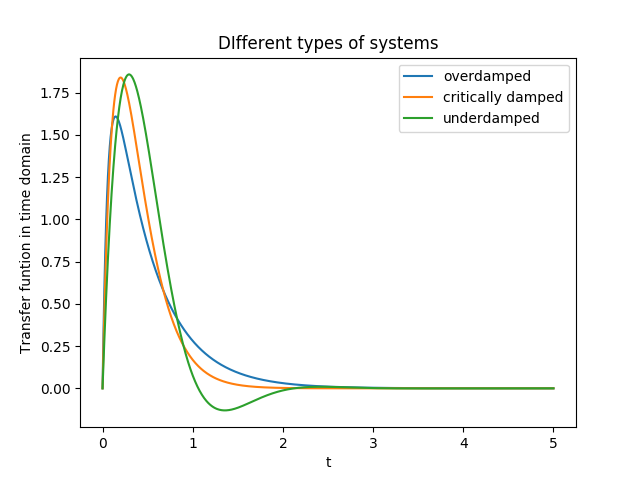
\includegraphics[width=0.7\linewidth]{Damping.png}
    \caption{Different systems based on \zeta}
    \label{fig:Graph}
\end{figure}
\end{frame}

\begin{frame}
    

\huge{\centerline{The End}}
\end{frame}

\end{document}
